% !TeX encoding = UTF-8
% !TeX program = xelatex
\documentclass[12pt, a4paper]{article}
\usepackage{xeCJK} % 须放在\usepackage{}列中足够前的位置
\usepackage{fontspec}
\usepackage{graphicx}
\usepackage{caption}
\usepackage{enumerate}
\usepackage{setspace}
\usepackage{array} % 製作表格必須的宏包
\usepackage{tabularx} % 自動調整列寬的表格宏包
\usepackage{adjustbox}
\setCJKfamilyfont{heiti}{Heiti TC}
\CJKfamily{heiti}
\setmainfont{Arial}
\setstretch{1.5}


\begin{document}
\begin{center}
  {\Huge 邏輯設計實驗} \\[2.5cm]
  {\Huge Lab10} \\[1.5cm]
  {\Huge 閂鎖器與正反器} \\ [4.5cm]
  \hspace{.6in}
  \begin{minipage}[t]{.4\linewidth}
    {\Large 班級:資訊一甲}\\[0.5cm]
    {\Large 學號:D1109023}\\[0.5cm]
    {\Large 姓名:楊孟憲}
  \end{minipage}    
\end{center}

\newpage
%\fontsize{30pt}{36pt}\selectfont 
%\normalsize

\begin{description}
  \fontsize{22pt}{25pt}\selectfont 
    \item [一、]摘要 
      \begin{enumerate}
        \fontsize{20pt}{22pt}\selectfont
          \item 組合邏輯與續向邏輯 
            \begin{description}
              \fontsize{16pt}{20}\selectfont
                \item [$\bullet$] 邏輯電路分為「組合邏輯」與「序向邏輯」兩類。
                \item [$\bullet$] 組合邏輯的輸出是「現在輸入」的函數,也就是說,有相同的輸入必然有相同的輸出。
                \item [$\bullet$] 序向邏輯中的輸出不僅是「現在輸入」的函數,同時也是「目前狀態」的函數;換言之,系統中必須擁有能將這些狀態記憶住的裝置,這就是閂鎖器/正反器的功能。\\
              \normalsize
            \end{description}
            \item 閂鎖器 
              \begin{description}
                \fontsize{16pt}{20}\selectfont
                  \item [$\bullet$] S  :資料設定(Data Set)
                  \item [$\bullet$] R  :資料重置(Data Reset)
                  \item [$\bullet$] 邏輯符號 \\[.5cm]
                  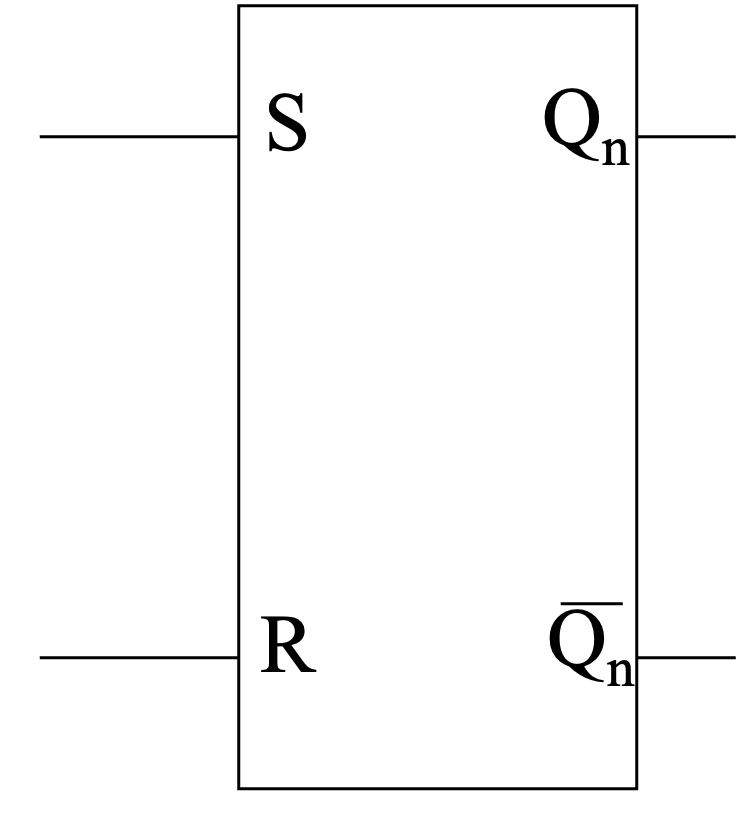
\includegraphics[width=5cm]{./image/latch.png} \\
                  \item[$\bullet$] 真值表 \\[.5cm]
                  
\includegraphics[width=10cm]{./image/latch_truthtable.png}
                \normalsize
              \end{description}

              \item D型閘控閂鎖器 \\
              \begin{description}
                \fontsize{16pt}{20}\selectfont
                  \item [(1)] 加法器: $X + Y = X +(Y + 0)$
                  \item [(2)] 減法器: $X - Y = X + (-Y) = X + (\bar{Y} + 1)$ \\
                \normalsize  
              \end{description}
            
              \item 實驗 \\
              \begin{description}
                \fontsize{16pt}{20}\selectfont
                  \item [(1)] D型 閂鎖器 (D Latch) 
                  \item [(2)] D型 正反器 (D Flip-Flop) 
                  \item [(3)] An 8-bit Register with asynchronous reset \\
                \normalsize  
              \end{description}

        \normalsize
      \end{enumerate}
    \item [二、]實驗結果
      \begin{description}
        \fontsize{20pt}{22pt}\selectfont
        \item 實驗 (四位元無號數加減法器)
          \fontsize{16pt}{18pt}\selectfont
            \begin{description}
              \item [$\bullet$]利用7483及XOR閘,實作一個四位元加減法器
              \item [$\bullet$]將A連接到固定的二進位數字(four bits), B連接到二進制的數字(four bits),以及一個 $m$ ($m=0$ repersent addition. otherwise, subtraction.)執行加減法運算, 並記錄其輸出總和S(binary)及進位輸出C4的值.\\
              \fontsize{18pt}{20pt}
                \item [(1)]電路圖 \\[.3cm]
                \begin{samepage}
                  \fontsize{16pt}{18pt}
                    當 m 為一時,代表 B 要轉成負數,並且因為 A 和 B 都是無號數,所以需要將 B 做 2 的補數。
                    \\這時候我們可以利用 XOR 閘來完成這項任務。\\[.5cm]
                    \bf{XOR 真值表}\\[.3cm]
                      \normalfont
                      \begin{tabular}{|c|c|c|}
                        \hline
                        A & B & Output \\
                        \hline
                        0 & 0 & 0 \\
                        \hline
                        0 & 1 & 1 \\
                        \hline
                        1 & 0 & 1 \\
                        \hline
                        1 & 1 & 0 \\
                        \hline
                      \end{tabular}
                      \\[.4cm] 觀察 XOR 真值表可以發現,任何數值對 1 做 XOR 會有反向的效果  $X \oplus 1 = X^{'}$。
                      \\ 所以可以利用 XOR 一端接到 m,一端接到輸入端,這樣子當 m 為零時(減法),就可以講 B 做 2 的補數了。\\
                \end{samepage}
    
                  \bf {電路圖} \\             
                  %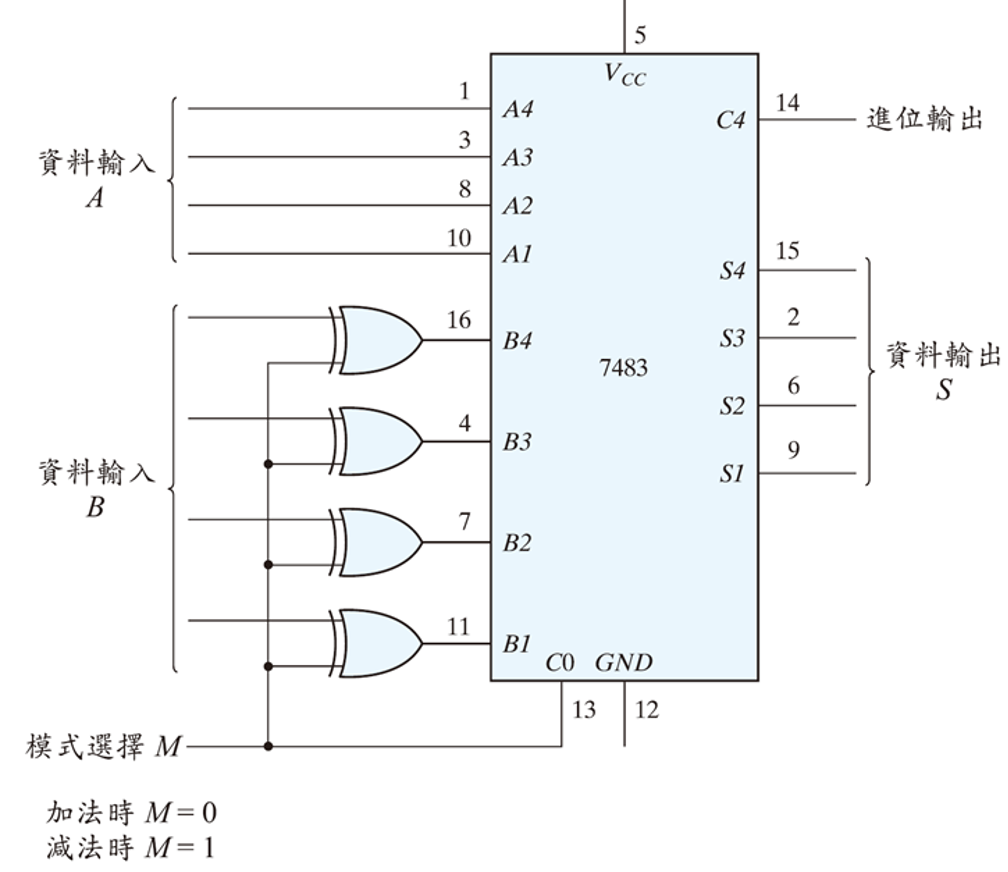
\includegraphics[width=12cm]{./image/7483.png}
                  \normalfont
              \item [(2)] Quartus II 軟體實做 DEO 電路板 \\[6cm]
              
              \begin{minipage}{\linewidth}
                \normalfont
                先將電路圖畫出後,再將相對應的腳位對上,編譯後完成。\\
                \bf{電路圖} \\[.4cm]
                %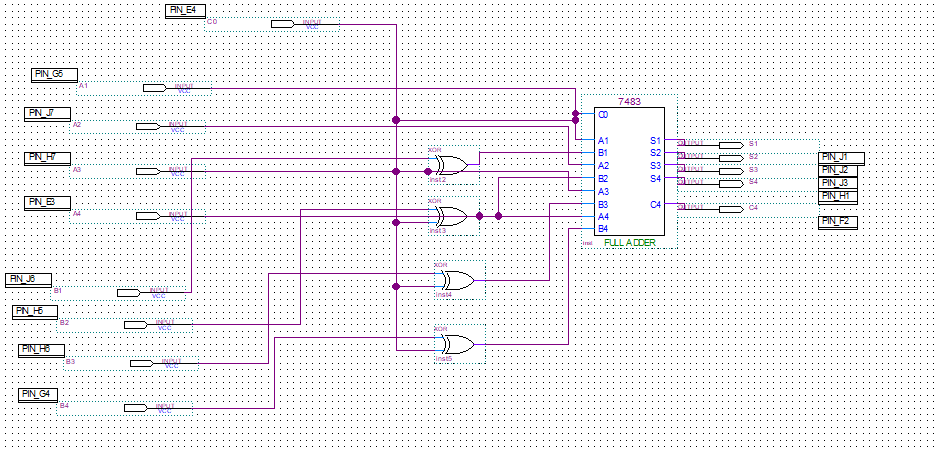
\includegraphics[width=12cm]{./image/Quartus-II.png}
              \end{minipage}
              
            \end{description}
          \normalsize  
        \normalsize
      \end{description}
    \item [三、]問題討論心得 \\[.6cm]
      \begin{minipage}[t]{\linewidth}
        \fontsize{16}{18}\selectfont
          這次實驗與以往不同,改用 DEO 電路板以及電路設計軟體 \bf{Quartus II} \normalfont 實做電路圖,並設定腳位。
          在前幾堂課程將邏輯閘基礎以及 K-map 基礎打好,學習新的工具比較能上手。這個工具也讓我們可以不用 Debug 硬體了,只要將電路圖畫好,大致上應該就沒有問題了。
          期待往後的實驗課程!
        \normalsize  
      \end{minipage}
  \normalsize
\end{description}

\end{document}

